%%%%%%%%%%%%%%%%%%%%%%%%%%%%%%%%%%%%%%%%%
% Dreuw & Deselaer's Poster
% LaTeX Template
% Version 1.0 (11/04/13)
%
% Created by:
% Philippe Dreuw and Thomas Deselaers
% http://www-i6.informatik.rwth-aachen.de/~dreuw/latexbeamerposter.php
%
% This template has been downloaded from:
% http://www.LaTeXTemplates.com
%
% License:
% CC BY-NC-SA 3.0 (http://creativecommons.org/licenses/by-nc-sa/3.0/)
%
%%%%%%%%%%%%%%%%%%%%%%%%%%%%%%%%%%%%%%%%%

%----------------------------------------------------------------------------------------
%	PACKAGES AND OTHER DOCUMENT CONFIGURATIONS
%----------------------------------------------------------------------------------------

\documentclass[final]{beamer}

\usepackage[utf8]{inputenc}

\usepackage[orientation=portrait,size=a0,scale=1.4]{beamerposter} % Use the beamerposter package for laying out the poster with a portrait orientation and an a0 paper size

\usetheme{I6pd2} % Use the I6pd2 theme supplied with this template

\usepackage[english]{babel} % English language/hyphenation

\usepackage{amsmath,amsthm,amssymb,latexsym} % For including math equations, theorems, symbols, etc

%\usepackage{times}\usefonttheme{professionalfonts}  % Uncomment to use Times as the main font
%\usefonttheme[onlymath]{serif} % Uncomment to use a Serif font within math environments

%\boldmath % Use bold for everything within the math environment

\usepackage{booktabs} % Top and bottom rules for tables

\graphicspath{{figures/}} % Location of the graphics files

\usecaptiontemplate{\small\structure{\insertcaptionname~\insertcaptionnumber: }\insertcaption} % A fix for figure numbering

%----------------------------------------------------------------------------------------
%	TITLE SECTION 
%----------------------------------------------------------------------------------------

\title{\LARGE Glottal inversion with an approximate vocal tract filter} % Poster title

\author{Lasse Lybeck, Robert Sirviö} % Author(s)

\institute{University of Helsinki, Department of Mathematics and Statistics} % Institution(s)

%----------------------------------------------------------------------------------------
%	FOOTER TEXT
%----------------------------------------------------------------------------------------

\newcommand{\leftfoot}{} % Left footer text

\newcommand{\rightfoot}{lasse.lybeck@helsinki.fi, robert.sirvio@helsinki.fi} % Right footer text

%----------------------------------------------------------------------------------------

\begin{document}

\addtobeamertemplate{block end}{}{\vspace*{2ex}} % White space under blocks

\begin{frame}[t] % The whole poster is enclosed in one beamer frame

\begin{columns}[t] % The whole poster consists of two major columns, each of which can be subdivided further with another \begin{columns} block - the [t] argument aligns each column's content to the top

\begin{column}{.02\textwidth}\end{column} % Empty spacer column

\begin{column}{.465\textwidth} % The first column


%----------------------------------------------------------------------------------------
%	INTRODUCTION
%----------------------------------------------------------------------------------------
            
\begin{block}{Introduction}

\begin{itemize}
\item A synthetic human vowel sound consists of a periodic signal to simulate the glottal excitation signal at the glottis and a filter to simulate the vocal tract, which the glottal signal is filtered through.\cite{touda} With a given vocal tract filter the direct problem is \emph{given a glottal excitation signal, create the vowel sound}. The inverse problem is \emph{given a (recorded) vowel sound, find the glottal excitation signal}. We will be concentrating on the inverse problem using simulated vowel data.

\item The inversion from a vowel sound to the glottal signal is an important part of creating synthetic human voices and speech generators. To create a synthetic vowel both the glottal signal and the vocal tract filter are needed. However, the glottal signal cannot be directly measured, but it can be approximated with inversion of a recorded vowel. This data can be used to create models for simulating the glottal excitation signal.
\end{itemize}

\end{block}

%----------------------------------------------------------------------------------------
%	METHODS
%----------------------------------------------------------------------------------------

\begin{block}{Methods}

\begin{columns} % Subdivide the first main column
\begin{column}{.54\textwidth} % The first subdivided column within the first main column

\begin{itemize}

\item The Rosenberg-Klatt model (\emph{RK-model)} \cite{rosenberg} was used to simulate the glottal excitation signal. An example of the resulting airflow and pressure can be seen in figure \ref{fig:klatt}.

\end{itemize}

\end{column}

\begin{column}{.43\textwidth} % The second subdivided column within the first main column

\begin{figure}[t]
\begin{center}
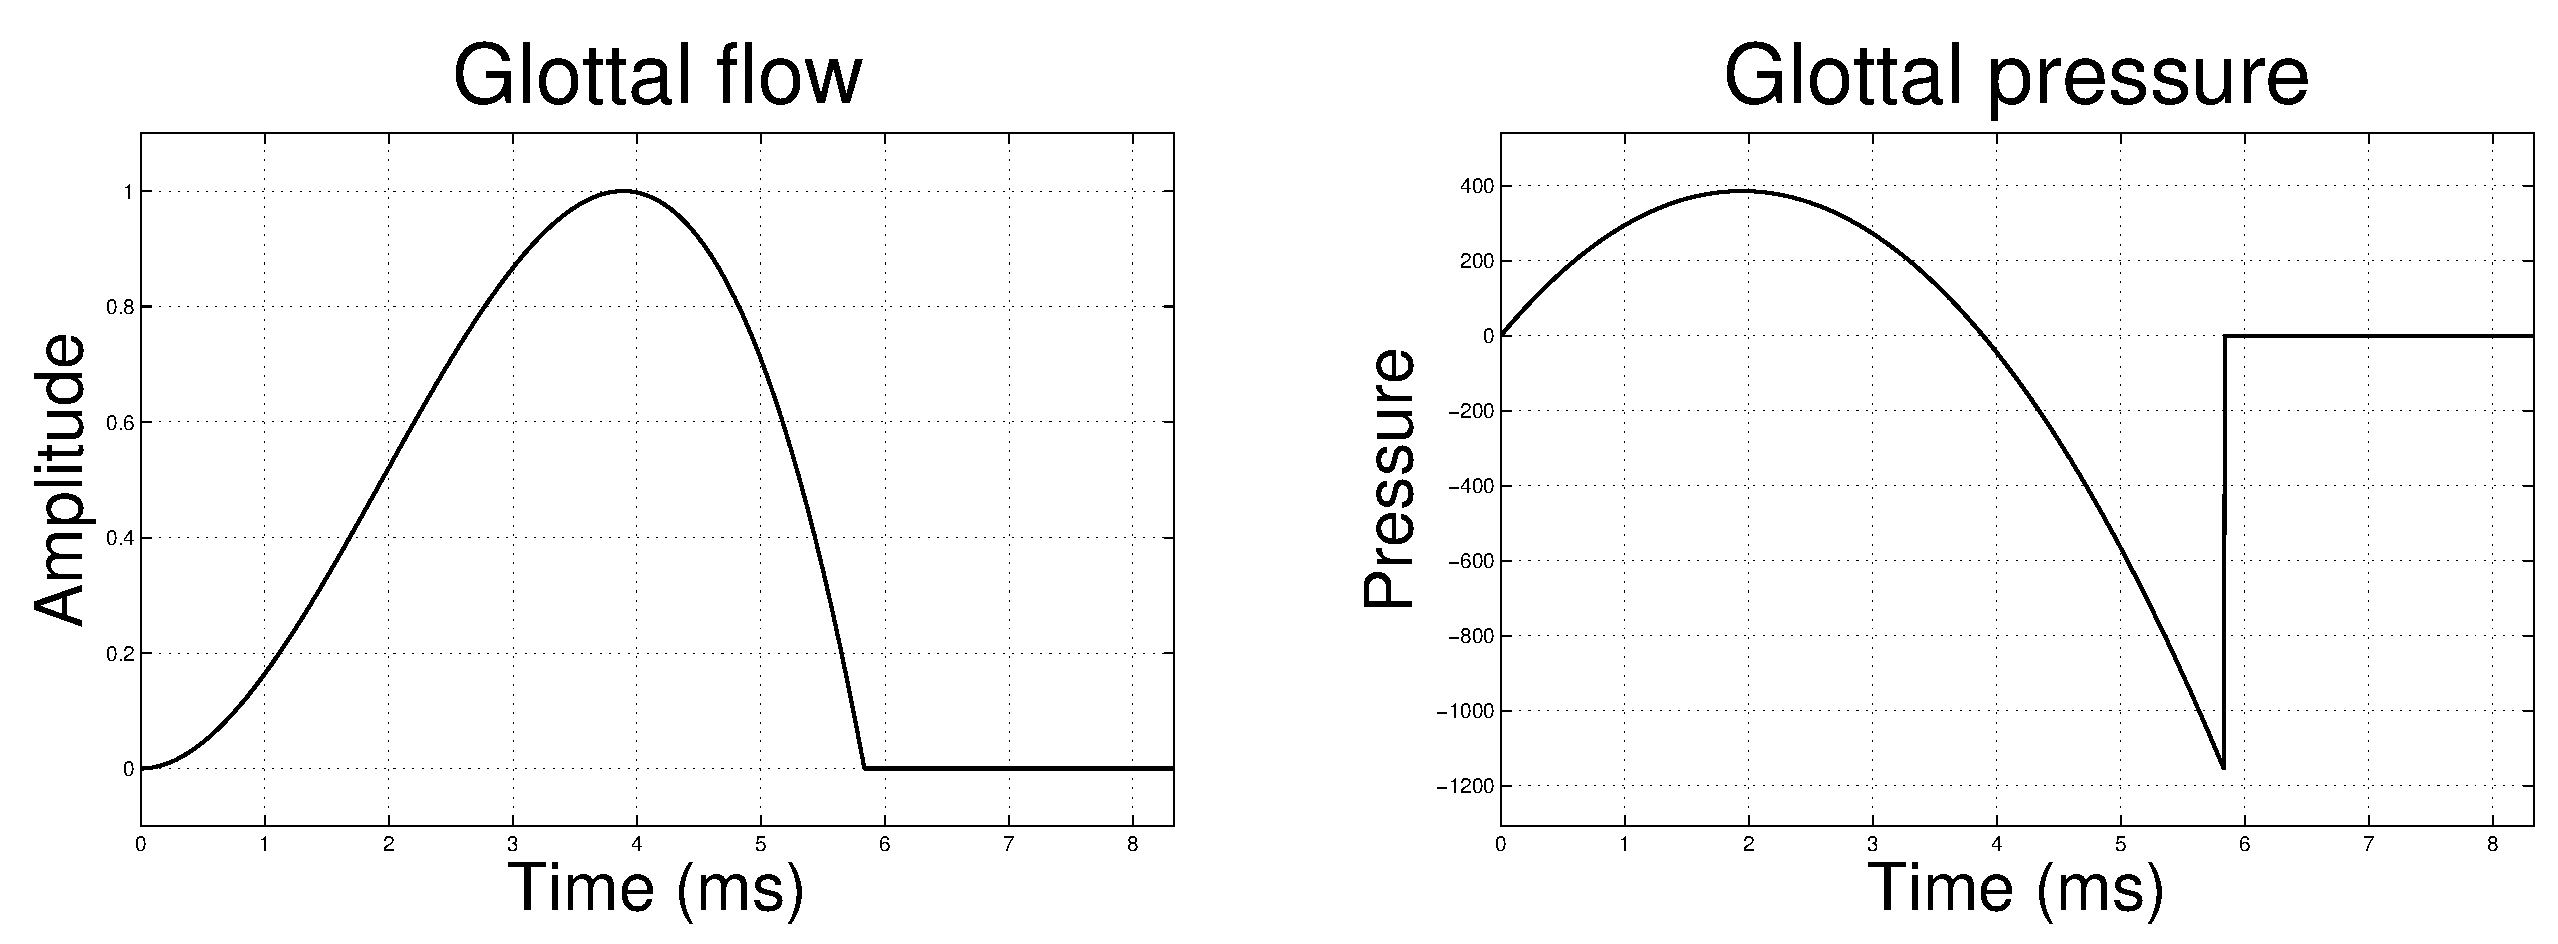
\includegraphics[width=\linewidth]{klatt.eps}
\end{center}
\caption{The airflow and pressure generated by the RK-model}
\label{fig:klatt}
\end{figure}

\end{column}
\end{columns} % End of the subdivision

\end{block}

%----------------------------------------------------------------------------------------
%	MATERIALS
%----------------------------------------------------------------------------------------

\begin{block}{Materials}

\begin{columns} % Subdivide the first main column
\begin{column}{.54\textwidth} % The first subdivided column within the first main column
\begin{itemize}
\item Vestibulum nisl, quis euismod velit eros in ligula.
\begin{itemize}
\item Cras rhoncus quam et augue convallis in elementum urna tincidunt.
\end{itemize}
\item Proin ut vestibulum augue.
\begin{itemize}
\item Donec dapibus sagittis neque eu ultrices.
\end{itemize}
\end{itemize}
\end{column}

\begin{column}{.43\textwidth} % The second subdivided column within the first main column
\centering
\begin{figure}

\includegraphics[width=0.8\linewidth]{placeholder.jpg}
\caption{Figure caption}
\end{figure}
\end{column}
\end{columns} % End of the subdivision

\begin{itemize}
\item Curabitur sapien ligula, faucibus in feugiat quis, vestibulum a turpis.
\begin{itemize}
\item Phasellus quis nunc neque. Suspendisse mauris diam, suscipit non gravida in, placerat id enim. Ut nec ipsum in lectus ultrices sagittis.
\item Ut nec ipsum in lectus ultrices sagittis.
\item Phasellus quis nunc neque.
\end{itemize}
\end{itemize}

\end{block}


%----------------------------------------------------------------------------------------

\end{column} % End of the first column

\begin{column}{.03\textwidth}\end{column} % Empty spacer column
 
\begin{column}{.465\textwidth} % The second column

%----------------------------------------------------------------------------------------
%	RESULTS
%----------------------------------------------------------------------------------------

\begin{block}{Results: Table}

\begin{itemize}
\item Ased Aliquet Luctus Lectus
\end{itemize}

\begin{table}
\begin{tabular}{l l l}
\toprule
\textbf{Treatments} & \textbf{Response 1} & \textbf{Response 2}\\
\midrule
Treatment 1 & 0.0003262 & 0.562 \\
Treatment 2 & 0.0015681 & 0.910 \\
Treatment 3 & 0.0009271 & 0.296 \\
\bottomrule
\end{tabular}
\caption{Table caption}
\end{table}

\begin{itemize}
\item Sollicitudin Vel Orci
\item Maecenas Ultricies Feugiat Velit Non Mattis.
\end{itemize}

\begin{table}
\begin{tabular}{l l l}
\toprule
\textbf{Treatments} & \textbf{Response 1} & \textbf{Response 2}\\
\midrule
Treatment 1 & 0.0003262 & 0.562 \\
Treatment 2 & 0.0015681 & 0.910 \\
Treatment 3 & 0.0009271 & 0.296 \\
\bottomrule
\end{tabular}
\caption{Table caption}
\end{table}
     
\end{block}

%------------------------------------------------

\begin{block}{Results: Figure}

\begin{figure}

\includegraphics[width=0.8\linewidth]{placeholder.jpg}
\caption{Figure caption}
\end{figure}

\end{block}

%----------------------------------------------------------------------------------------
%	DISCUSSION
%----------------------------------------------------------------------------------------

\begin{block}{Discussion}



\end{block}

%----------------------------------------------------------------------------------------
%	REFERENCES
%----------------------------------------------------------------------------------------

\begin{block}{References}

\begin{scriptsize}


\begin{thebibliography}{9}

\bibitem{fant}
    Fant, G., Liljencrants, J., Lin, Q., (1985).
    \emph{A four-parameter model of glottal flow}.
    STL-QPSR 26 (4), p. 1-13
    
\bibitem{fujisaki}
    Fujisaki, H., Ljungqvist, M., 1986.
    Proposal and evaluation of models for the glottal source waveform.
    In: Proc. IEEE International Conference on Acoustics, Speech and Signal Processing (ICASSP). Vol. 11. p. 1605–1608.
    
\bibitem{samu}
	Mueller, Jennifer L. \& Siltanen Samuli, (2012).
	\emph{Linear and Nonlinear Inverse Problems with Practical Applications}.
	SIAM, 1:st edition.
	
\bibitem{touda}
    Touda, K., (2007)
    \emph{Study on numerical method for voice generation problem}.
    PhD thesis.
    The University of Electro-Communications.
    
\bibitem{digitalmodels}
    Rabiner, L. R., Schafer, R. W., (1987).
    \emph{Digital processing of speech signals}.
    Englewood Cliffs: Prentice-Hall, p. 38-107.

\bibitem{rosenberg}
    Rosenberg, A., (1971).
    \emph{Effect of glottal pulse shape on the quality of natural vowels}.
    Journal of the Acoustical Society of America 49 (2B), p. 583–590.

\end{thebibliography}

%\nocite{*} % Insert publications even if they are not cited in the poster
%\small{\bibliographystyle{unsrt}
%\bibliography{sample}}

\end{scriptsize}

\end{block}


%----------------------------------------------------------------------------------------

\end{column} % End of the second column

\begin{column}{.015\textwidth}\end{column} % Empty spacer column

\end{columns} % End of all the columns in the poster

\end{frame} % End of the enclosing frame

\end{document}